\begin{appendices}

\chapter{Parsers performance benchmarks}

We performed the performance evaluation of the restricted Markdown"/like language parsers
implemented using the designed libraries.

The benchmarks compare three parsers: the first one is implemented with our monad
transformers parsing library; the second parser is one build with extensible effects
library; and the third is the Markdonw parser of the highly"/popular and
industry"/recognised Pandoc document converter. The results of the benchmarking show
that the first parser is the fastest, even faster that Pandoc. This is probably because of
it's high specialisation. The extensible effects parser is dramatically slower than
the monad transformers one. The problem of performance of free monads based programmes
is addressed by Kiselyov at al.~\cite{Kiselyov:2015:FMM:2887747.2804319}.
The free monads need to have more efficient implementation in order to
compete with monad transformers for performance.

The rest of this appendix is a report generated by~\emph{criterion}~---
a Haskell benchmarking library. The report contains the mean values of the
execution time, corresponding standard deviations and the execution time plots.
The section ``understanding this report'' contains the detailed information on
every entity in the report. The source code of the benchmarks is available on
GitHub~\cite{parsers-benchmarks}.

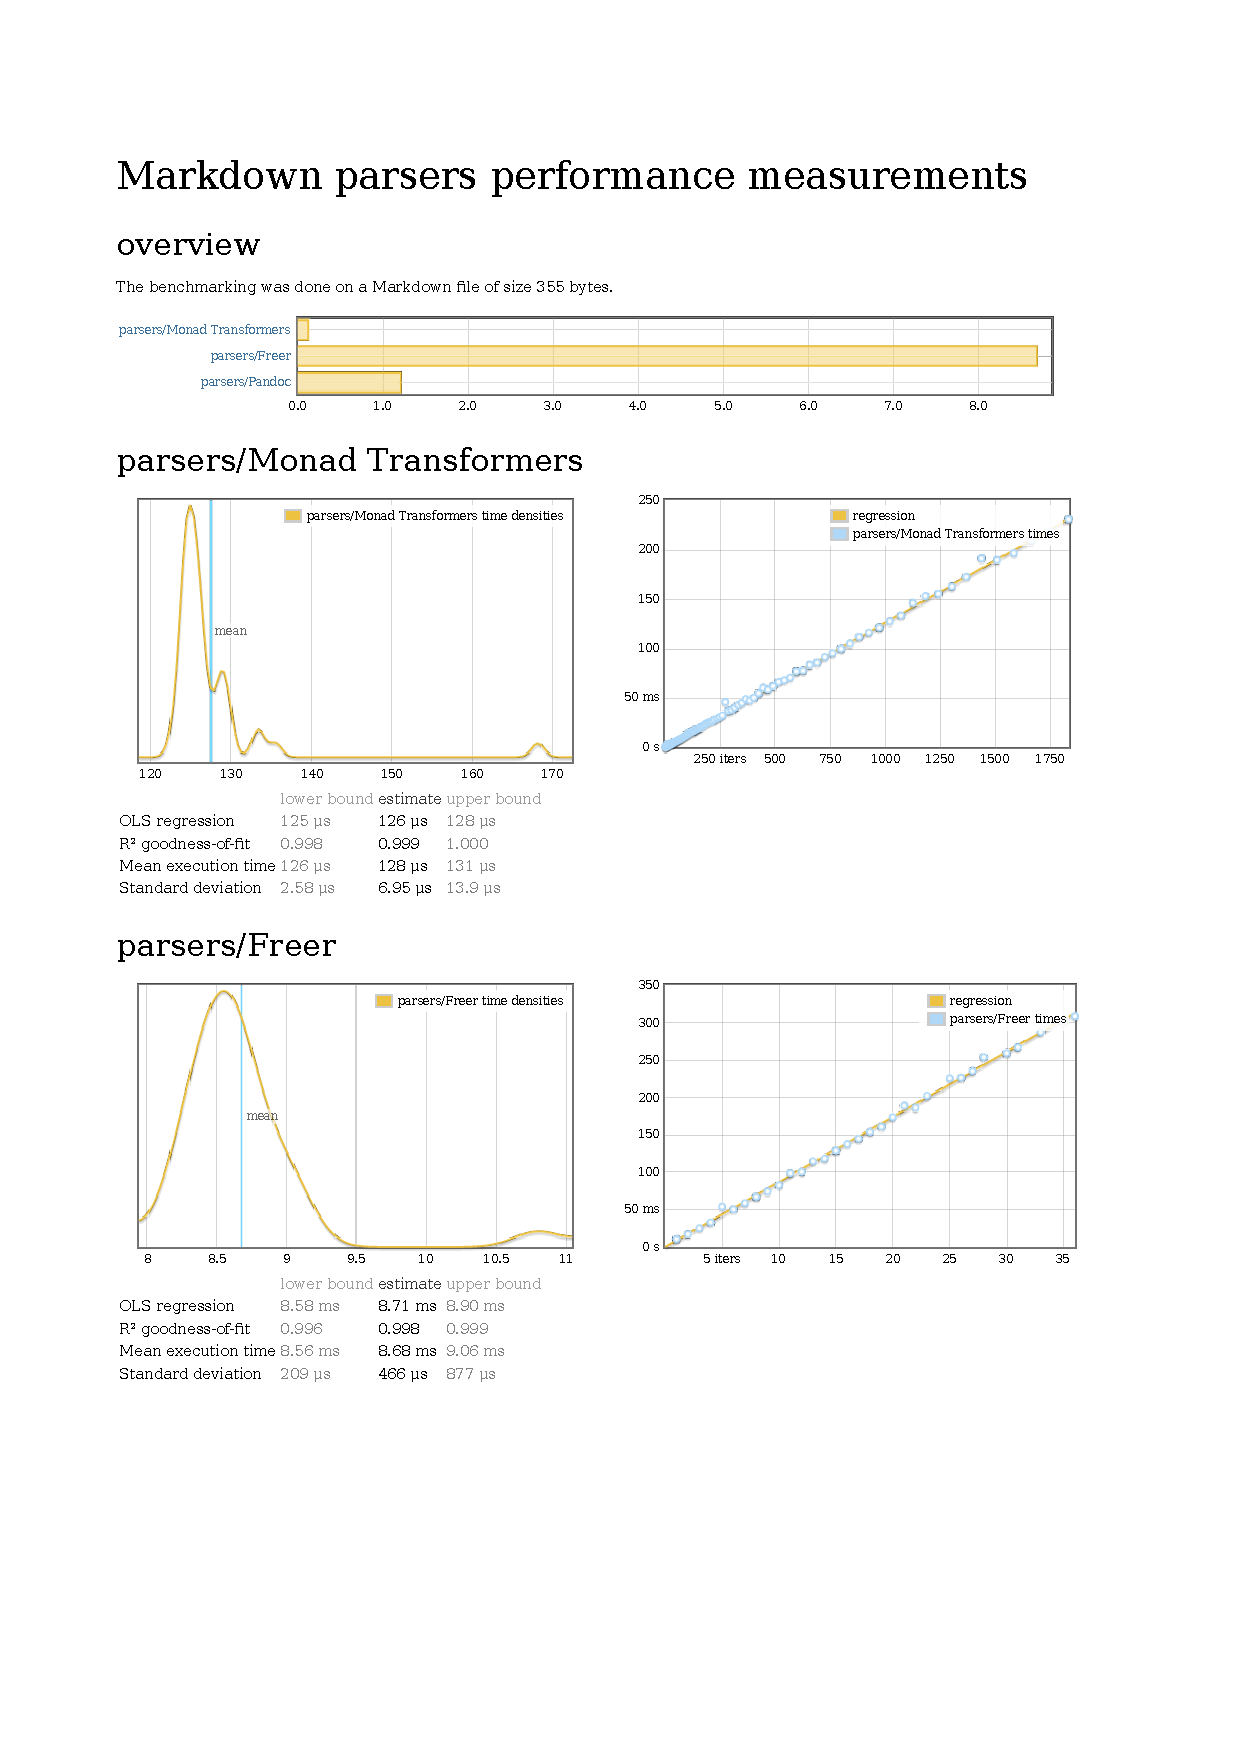
\includepdf[pages=-]{images/benchmark-report.pdf}

\end{appendices}